\documentclass[11pt,bibliography=totoc]{scrartcl}

% Son titrage
\author{Juan-Carlos Barros et Daniel Kessler}
\date{\today}
\title{Conception d'une séquence d'enseignement\\\medskip
  \large GymInf, Didactique de l'informatique, Rendu 010}

% son français
%\usepackage{csquotes}
\usepackage[french]{babel}

% Sa gestion de bibliographie
% NB: nos consignes nous demandent d'utiliser les normes APA
%     ça tombe bien, c'est possible de le préciser ici!
\usepackage[backend=biber,style=apa,
            urldate=edtf,date=edtf,seconds=true]{biblatex}
\addbibresource{biblio.bib}

% configuration générale
\usepackage[l2tabu, orthodox]{nag}  % demander indication d'usages désuets
\usepackage{microtype}  % subtiles améliorations de certains défauts
\usepackage[french]{babel}  % langue du document
\usepackage{graphicx}  % pour inclure des images et des pdf
\usepackage{array} % pour les tableaux?
\usepackage{booktabs}  % pour des tablulars plus jolis
\renewcommand{\arraystretch}{1.2}

% configuration des polices de caractère / aspect du titre
\usepackage[utf8]{inputenc}  % nécessaire en MS-Windows, pas dans Linux
                             % (probablement pas dans MacOS non plus)
% Possibles changements de police ci-dessous (en décomenter un, ou pas)
\usepackage[T1]{fontenc}  % <- c'est nécessaire dans window$, je crois
% \usepackage{tgtermes} %  (semble nécessiter lualatex)

% configuration géométrie / en-tête / pieds de page
% remplacer 2.2 par 1.2 ci-dessous avec scrartcl (mise en page de base différente)
\addtolength{\voffset}{-2.2cm}   % reprendre la place de l'en-tête inexistante
\addtolength{\textheight}{4.2cm} % laisser plus de place pour le pied de page
\usepackage[compatV3]{fancyhdr}  % gestion d'en-tête et pied de page
\pagestyle{fancy}
\renewcommand\headrulewidth{0pt}   % pas de barre sous en-tête
\renewcommand\footrulewidth{0.4pt} % barre sur pied de page
\usepackage{lastpage}
\lfoot{pièce 010} \cfoot{} \rfoot{page \thepage/\pageref{LastPage}}
\fancypagestyle{plain}{  % style pour page de titre (pas de bas de page)
  \fancyhf{}\fancyfoot{}\renewcommand\footrulewidth{0pt} % barre sur pied de page
}
% pdfisation avec liens un peu bleus mais pas trop
\usepackage[pdfstartview=FitH,
pdfauthor={Juan-Carlos Barros et Daniel Kessler},
pdftitle={Conception d'une séquence}]{hyperref}
\usepackage{xcolor}
\definecolor{pdflinkcolor}{RGB}{30,60, 120}
\hypersetup{colorlinks=true, allcolors=pdflinkcolor}

% ses ajouts post-relecture
\newcommand\ajout[1]{{\color{blue} #1}}
\newcommand\rajout[1]{{\color{green} #1}}
\newcommand\rajouts[1]{{\color{cyan} #1}}

\begin{document}
\thispagestyle{plain}  % page de garde sans bas de page

% Démarrage avec titre et table des matières sur page séparée
\maketitle
\tableofcontents  % <- au début, on n'est pas des frouzes qui mettent ça à la fin...
\vfill
Code des couleurs:
\begin{itemize}
\item \ajout{modifications/ajouts suite à commentaires des pairs}\par
\item \rajout{modifications/ajouts suite à commentaires du formateur}\par
\item \rajouts{modifications/ajouts suite à commentaires des pairs et du formateur}\par
\end{itemize}
\vfill
\pagebreak

% Et c'est parti pour du contenu!
\section{Contexte institutionnel et disciplinaire}
Nous enseignons tous deux au niveau gymnasial dans le Collège de Genève
(Gymnase). Dans ce cadre, nous avons cette année plusieurs groupes d'élèves de
1ère année informatique discipline fondamentale, auxquels s'adresse le travail
présenté dans ce document. Ces groupes sont constitués de 16 élèves au maximum,
issus potentiellement de plusieurs ``classes'', OS, etc.  (le concept de
``classe'' est très flou au Collège, les élèves changeant souvent de groupe).
\ajout {On ne peut donc pas compter sur un ``profil'' homogène des élèves pour notre séquence.}

La séquence d'enseignement que nous allons présenter possède deux
caractéristiques originales:
\begin{itemize}
\item Elle se déroule sur plusieurs leçons (minimum  6), en prenant 20-30 minutes du cours à
  chaque fois.
\item Elle combine des objectifs explicites pour les élèves avec des objectifs
  implicites qui seront explicités plus tard.
\end{itemize}

Cette séquence s'insère en deuxième partie du premier semestre, après avoir
travaillé sur le code binaire, vu quelques encodages simples (nombres entiers,
caractères \textsc{ascii}, bitmaps) et travaillé un petit peu sur les composants
matériels d'un ordinateur, éléments du chapitre \textit{Information et Données}
du plan d'étude cantonal genevois \autocite{pecinfo}.

L'objectif explicite initial sera développé dans la partie
suivante. L'originalité de cette séquence repose sur le deuxième
objectif. Celui-ci consiste à découvrir la puissance des outils informatiques de
collaboration pour déboucher finalement sur un exemple iconique:
\textit{Wikipedia}.

Ce deuxième objectif participe à plusieurs thèmes du plan d'étude, notamment les
\textit{Réseaux}, \textit{Information et Données} et la \textit{Citoyenneté
  Numérique}.

\section{Objectifs pédagogiques}
L'objectif ``alibi'' (ou explicite) de la séquence présentée dans ce document
est d'approfondir un des éléments précédents, à travers un travail de groupe sur
un sujet vu ``de haut'' et pour lequel on aimerait avoir des approfondissements
sur certaines parties particulièrement intéressantes.  Par exemple, dans notre
cas, nous avons décidé d'approfondir la représentation des données à travers
l'étude de l'encodage des nombres à virgule flottante, des nombres relatifs, des
caractères avec notamment \textsc{utf}-8, des images en couleur, etc.).
Toutefois, il faut bien comprendre que cette séquence est adaptable et peut
s'intercaler où l'on veut dans l'année car il suffit de choisir des sujets de
projets en lien avec le(s) dernier(s) chapitre(s) abordé(s). Cela permet de ne
pas trop s'attarder sur des notions qui pourraient autrement prendre beaucoup de
place dans le planning des leçons; elles seront prémâchées à travers les projets
``par les élèves, pour les élèves''.

L'objectif principal, quant à lui, repose sur la découverte des outils de
collaboration. On veut amener les élèves à en apercevoir le potentiel.  On fera
donc utiliser aux élèves un \textit{wiki} pour partager le fruit de leur
recherche explicite.  Ce n'est qu'en fin de séquence qu'on leur fera découvrir
que certains wikis sont très ouverts aux contributions publiques, notamment
\textit{Wikipedia}.  Après avoir expérimenté le travail sur un wiki, un élève
devrait comprendre le mécanisme de base et se sentir capable de contribuer à
\textit{Wikipedia}, que ce soit en repérant une coquille à corriger, une
information caduque ou incomplète, voire en produisant de nouvelles pages.

\rajouts {
Voici un tableau synthétisant les principaux objectifs ``implicites'' concernés par cette séquence:
\begin{center}
   \begin{tabular}{@{}lm{.35\textwidth}m{.35\textwidth}@{}}\toprule
     Activité & Objectifs %(généraux ou terminaux)
     & Indicateurs (évaluation) \\ 
     \midrule
     Introduction & Savoir s'organiser au sein d'un groupe & Formulaire correctement renseigné \\ 
     Documentation & Savoir trier les informations utiles & Choix des sources et arguments de validation \\
     Reformulation & Savoir adapter des sources au niveau du public & Commentaires des pairs \\
     Utilisation des wikis & Savoir utiliser un outil de collaboration & Observation du groupe, résultat \\
     \bottomrule
   \end{tabular}
 \end{center}
}

\rajout{Selon le choix des sujets, divers objectifs directement en lien avec le
  \cite{pecinfo} seront aussi présents. La liste ci-dessous indique certains
  éléments ayant émergé de certains travaux d'élèves lors de la première mise en
  oeuvre de cette séquence:
\begin{itemize}
\item concernant la \textit{représentation numérique de l'information}:
  \begin{itemize}
  \item distinguer une donnée \textit{analogique} (continue) d'une donnée
    \textit{digitale} (discrète) [avec le sujet ``encodage du son'']
  \item ``distinguer les avantages et inconvénients'' de certains
    encodages [avec le sujet ``encoder des caractères hors-ASCII'']
  \item ``comprendre que l'ordinateur encode de différentes
    manières'' [avec les sujets ``encodage des nombres entiers
    relatifs'' et ``encodage des nombres à virgule flottante'']
  \item ``identifier le rôle des composants principaux d'un ordinateur'' [avec
    le sujet ``composants d'un smartphone'']
  \end{itemize}
\end{itemize}
}

\section{Scénario d'apprentissage}
Les élèves seront amenés à travailler entre 20 et 30 minutes chaque semaine,
pendant 6 semaines, sur leurs projets. Le travail s'effectue en grande partie
autour de la conception d'un wiki par chaque groupe. Une fois ce travail achevé,
une transposition est effectuée du mode de travail employé par les élèves vers
la manière dont fonctionne Wikipedia, en clarifiant que les élèves sont
maintenant habilités à y contribuer s'ils le souhaitent.

Voici le calendrier général de la séquence.
\begin{center}
\begin{tabular}{rp{.7\textwidth}}
  semaine 1& les groupes et les sujets sont définis\\
  semaine 2& le wiki du groupe a au moins 2 pages différentes et 3 liens
             externes vers des sources;
             la répartition des tâches au sein du groupe (qui fait quoi) est claire et documentée\\
  semaine 3& toutes les informations utiles ont été trouvées et répertoriées
             (liens vers sources);
             un élève d'un autre groupe devrait pouvoir bien comprendre le sujet grâce à ce wiki\\
  semaine 4& chaque élève a lu le wiki d'un autre groupe et fourni des commentaires utiles à celui-ci\\
  semaine 5& le wiki est fini et complet, en prenant en compte les remarques des
             camarades d'autres groupes qui l'ont lu\\
  semaine 6& présentation orale (10 min) en se servant du wiki \\
% dommage de ne pas privilégier le Wiki ici: 
% pourquoi leur proposer de présenter à l'aide d'un autre outil?
% ça c'est le problème d'avoir copié-collé mon machin fait avant qu'on décide de
% se projet => je change ici *et* dans la version pour mes élèves  
  semaine 7& debriefing et présentation de Wikipedia
\end{tabular}  
\end{center}

Nous pouvons découper le scénario d'apprentissage en cinq étapes, en suivant le
modèle de Robert Bibeau \autocite{bibeau}.

\subsection{Mise en situation}
L'enseignant explique à la classe que tout en démarrant un nouveau thème de
travail, le thème précédent sera approfondi par des travaux de groupe auxquels
20 à 30 minutes de temps du cours seront consacrés pendant les 6 prochains cours.
La première semaine, il est juste question de constituer des groupes, choisir un
sujet et effectuer une brève recherche préliminaire de sources. Il n'est pas
encore explicitement question de wiki (éviter la surcharge cognitive: pour
l'instant, on cherche un sujet et on essaye de constituer des groupes d'élèves
pouvant fonctionner ensemble de manière efficace et agréable).

\rajout{Avant de commencer, l'enseignant récapitule brièvement ce qui a été déjà
  vu sur la thématique de la représentation des données et donne quelques
  exemples de questions restées ouvertes et d'encodages importants qui n'ont été
  qu'effleurés mais pas traités en détail, constituant ainsi des sujets
  possibles pour les futurs projets.}  Les groupes d'élèves sont constitués et
un sujet choisi par chacun (cf. Annexe \ref{annexe:groupes}). Les élèves sont
invités à choisir un élément de la partie du cours précédent qu'ils souhaitent
approfondir. Le rôle de l'enseignant à cette étape est de se balader entre les
groupes et s'assurer que chacun arrive à choisir un thème qui est pertinent pour
le cours et intéresse réellement les élèves du groupe. \ajout{Il donne des
  conseils sur l'organisation: délégation de tâches, domaines de compétences de
  chacun, etc.}

\subsection{Situation d'apprentissage}
Les élèves ont accès assez vite à une version en-ligne du calendrier des
objectifs minimaux à atteindre chaque semaine pour les semaines 2 à 6
\rajout{(cf. Annexe \ref{annexe:calendrier})}. Ce calendrier peut être adapté
suivant les éventuels imprévus.

Une fois les groupes constitués, un moment ``frontal'' d'une dizaine de minutes
est utilisé par l'enseignant pour montrer aux élèves les rudiments du
fonctionnement du wiki sur Moodle (notamment comment créer un lien vers une
autre page du wiki, déjà existante ou pas, et comment créer un lien vers une
\textsc{url} externe). \ajout {Les élèves peuvent (selon le choix de
  l'enseignant) tester en direct les notions montrées par l'enseignant. Les
  erreurs arrivent naturellement assez vite, ce qui permet à l'enseignant de
  détailler les explications selon le degré d'acquisition des élèves.}

Les élèves sont invités à travailler 20 à 30 minutes chaque semaine sur leur
projet, avec des objectifs minimaux chaque semaine. Aucun ``devoir à la maison''
explicite n'est donné, mais il est indiqué que s'ils le souhaitent, ils peuvent
avancer sur leur projet en dehors des heures de cours.

\rajout{Pendant ces périodes, l'enseignant se balade entre les groupes, observe
  leur travail et intéragit avec eux afin d'encourager et valider leurs méthodes
  de travail plutôt que les informations trouvées. Cette démarche se rapproche
  un peu de la méthode \textsc{pogil} (Process Oriented Guided Inquiry Learning,
  cf. \url{https://pogil.org}).}

\subsection{Objectivation}
Chaque élève est amené à évaluer le wiki d'un autre groupe lors de la semaine
4. Cette étape devrait lui permettre de se détacher de son propre travail,
prendre du recul et y revenir avec un regard neuf. De plus, cette étape permet
une évaluation formative par les pairs. Chaque élève se voit assigner le wiki
d'un autre projet lors de la semaine 4. Il reçoit à cet effet une feuille dont
le modèle se trouve à l'Annexe \ref{annexe:pairs}. Il devra laisser au moins
trois commentaires constructifs dans le wiki qui lui est assigné, et remplir et
rendre la feuille qui lui a été fournie, en montrant notamment en quoi la
navigation d'un autre wiki lui aura donné des idées pour son propre projet.
\ajout {L'enseignant a le rôle de s'assurer que les élèves comprennent bien le
  leur. C'est-à-dire que leurs commentaires doivent être bienveillants mais
  toutefois réalistes et constructifs pour permettre une double amélioration:
  celle du wiki évalué, bien entendu, mais également celle de leur propre wiki,
  suite à la comparaison entre celui-ci et celui qui est évalué.}

\subsection{Situation d'évaluation}
L'évaluation notée (donc ``sommative'') de cette séquence prend en compte trois
groupes de critères distincts:
\begin{itemize}
\item l'atteinte des objectifs minimaux à la fin de chaque semaine (sorte de
  ``contrôle continu'', évaluant la motivation et l'autonomie du groupe)
\item le wiki ``finalisé'' (entre guillemets parce qu'il peut encore être édité
  après: c'est bien un des buts de travailler avec un wiki!). \rajout{Celui-ci
    est évalué aussi bien sur la forme que sur le fond.}
\item la présentation orale (semaine 6)
\end{itemize}
\rajout{Une période de remédiation peut en outre être prévue après une première
  évaluation notée. Elle permet aux groupes qui le souhaitent d'améliorer leur
  wiki (forme et contenu) après leur présentation orale (dont un aspect
  important est constitué des questions de leurs camarades -- il est conseillé
  d'imposer un quota minimal d'une question de la part de chaque autre
  groupe). Cette remédiation éventuelle a lieu après avoir reçu une première
  évaluation chiffrée et des commentaires écrits de la part de l'enseignant, et
  elle ne concerne que le wiki lui-même. Les points donnés au \textit{contrôle
    continu} et à la présentation orale ne peuvent en revanche plus être
  modifiés. Cette étape est l'occasion de clarifier les critères d'évaluation du
  \textit{fond} et de la \textit{forme} du wiki en prenant aussi en compte les
  réactions des camarades lors des phases de \textit{commentaire d'un autre
    wiki} et \textit{questions pendant la présentation orale}, ainsi que les
  commentaires plus formels de l'enseignant.}

Le détail des critères se trouve dans l'Annexe \ref{annexe:grille}. Il est
modelé partiellement sur les critères d'évaluation officiels du Travail de
Maturité. D'ailleurs, le mode de travail et d'évaluation devrait permettre aussi
de donner aux élèves de 1ère année un avant-goût d'un TM de type ``travail de
recherche'' dans un domaine scientifique (ce qui peut être explicité à la fin).

\subsection{Situation de réinvestissement}
En tant qu'épilogue à la séquence, une discussion collective est lancée
concernant l'encyclopédie en-ligne Wikipedia: pourquoi ce nom? est-ce bien un
wiki comme ceux que les élèves ont investi pendant 5 semaines? qui peut
l'éditer? qui peut y écrire des commentaires?

Une activité sur Wikipedia pourra être lancée à ce moment, en fonction du temps
et des choix pédagogiques de l'enseignant.  On pourrait imaginer de lancer les
élèves à la chasse aux informations incorrectes ou manquantes dans des articles
de Wikipedia dont le contenu fait partie du domaine d'expertise de l'élève
chasseur. Un des domaines d'expertise pourrait être la connaissance de leur
établissement scolaire, dont l'article Wikipedia pourrait être améliorable voire
inexistant.  Dans un deuxième temps, une modification des articles pourra être
faite, soit de manière centralisée à travers l'enseignant, soit de nouveau par
petits groupe, sous la forme de mini projets ``amélioration de Wikipedia''.
\ajout {Un atelier ``création de nouvelle(s) page(s) Wikipedia'' peut également
  être réalisé pour enrichir la connaissance globale et mettre en valeur les
  connaissances de nos élèves. Si l'imagination manquait, on pourrait tout de
  même traduire des articles intéressants (par exemple articles informatiques
  liés aux thèmes abordés par les élèves dans leur Wikis) de l'anglais vers le
  français. Ceci pourrait d'ailleurs donner lieu à une collaboration
  transdisciplinaire avec un enseignant d'anglais. Malheureusement, avec les
  groupes d'élèves hétérogènes que nous avons, les élèves se retrouveront dans
  plusieurs cours d'anglais différents, ce qui compliquera sa réalisation mais
  ce serait probablement possible dans des établissements avec des
  groupes-classe compacts.  }

Conclusion prévue quelle que soit la teneur de l'``épilogue'' à cette séquence:
les élèves pourront par la suite, en tant que ``citoyens numériques'',
contribuer à Wikipedia s'ils le souhaitent. Ils auront eu une première
expérience de travail avec plusieurs wikis et seront donc compétents pour le
faire.

\section{Courant et stratégie pédagogiques}
Une bonne partie de la séquence proposée est appelée à se dérouler sous forme de
``petites équipes pour permettre l'apprentissage par les pairs et la
collaboration'', ce qui d'après Anastassis Kozanitis (\cite{kozanitis})
correspond au modèle socio-constructiviste. Kozanitis rappelle par ailleurs que
dans ce modèle didactique, ``l'enseignant doit veiller en permanence les [sic]
productions de l'étudiant et ses processus d'apprentissage''.  Par ailleurs,
quelques parties ``frontales'' sont également nécessaires, notamment vers le
début pour présenter l'outil (le wiki dans Moodle) et à la fin pour l'épilogue
(lien avec Wikipedia).

Quant aux niveaux des connaissances abordées, ils évoluent sur deux plans
parallèles.

\subsection{Plan des sujets explicites: encodage, etc.}
Dans le plan des connaissances ``externes'' étudiées puis transmises (sujet des
projets de chaque groupe), des connaissances doivent être acquises, mémorisées,
puis analysées et comprises par les élèves pour être finalement reformulées et
restituées à leurs pairs. Si on ajoute la connaissance procédurale consistant en
la mise en place d'exemples explicatifs de leur sujet de recherche (par exemple,
encodage et décodage d'un nombre à virgule flottante) et la connaissance
meta-cognitive (évaluation de leur sujet d'apprentissage afin d'en transmettre
les avantages et inconvénients), on peut constater qu'on traverse tous les
niveaux taxonomiques de Bloom (cf. \cite{bloom}), ce qui rend la méthode de cette séquence
particulièrement intéressante. 
\ajout{
Voici de manière synthétique les différents niveaux de la taxonomie de Bloom mis en jeu pour les objectifs ``explicites'':}
\rajout{
\begin{center}
   \begin{tabular}{@{}m{.2\textwidth}m{.18\textwidth}m{.5\textwidth}@{}}\toprule
     Activité élève & Niveau (Bloom) & Exemple(s) \\ 
     \midrule
     Apprentissage des connaissances & ``Remember'' et ``Understand'' & Mémorisation / Compréhension pour transmettre / expliquer ces connaissances aux camarades \\ 
     Production d'exemples & ``Apply'' & Mise en pratique des notions sur un exemple explicatif \\
     Critique du savoir acquis & ``Analyse'' et ``Evaluate'' & Capacité d'un
                                                               regard critique
                                                               vis-à-vis du
                                                               travail d'un
                                                               autre groupe (complexité, utilité, etc.) \\
     \bottomrule
   \end{tabular}
 \end{center}
}

\subsection{Plan des sujets implicites: Wikis -> Wikipedia -> Open Source}
Dans le plan de l'outil utilisé pour collaborer et transmettre l'information,
l'outil employé pour gérer l'acquisition mais surtout le partage et la
retransmission des connaissances (le wiki) devient à son tour une source de
connaissance.  Pour ce deuxième but implicite, la navigation dans les niveaux
est bien différente: On commence par les connaissances procédurales avec
l'utilisation des wikis de groupe puis on s'attaque aux autres niveaux de
connaissance: premièrement basiques avec l'apport de l'enseignant qui présente
Wikipedia puis de haut niveau avec les retours ``philosophiques'' sur
l'importance de Wikipedia et, plus largement, des courants \textit{open source},
\textit{logiciel libre}, etc.  \ajout{Voici de manière synthétique les
  différents niveaux de la taxonomie de Bloom mis en jeu pour les objectifs
  ``implicites'':}
\rajout{
\begin{center}
   \begin{tabular}{@{}m{.25\textwidth}m{.2\textwidth}m{.45\textwidth}@{}}
     \toprule
     Activité & Niveau (Bloom) & Exemple(s) \\ 
     \midrule
     Utilisation des Wikis & ``Apply'' & Essais/erreurs pour utiliser l'outil de manière efficace \\ 
     Théorie sur Wikipedia & ``Remember'' et ``Understand'' & Explication
                                                              ``frontale'' de
                                                              l'enseignant pour
                                                              expliquer le
                                                              fonctionnement
                                                              d'un wiki et ce
                                                              qu'est Wikipedia \\
     Analyse plus large & ``Analyse'' et ``Evaluate'' & Compréhension des enjeux
                                                        sociétaux, du courant
                                                        ``open'', du rôle des outils dans cette ``philosophie'' \\

     Optionnel: étape wikipedia & ``Create'' & Il faudrait nettement plus de
                                                 temps pour que les élèves
                                                 puissent créer un contenu
                                                 totalement original sur un
                                                 autre sujet\\
%     - & ``Create'' & Il faudrait consacrer nettement plus de temps pour que les élèves créent des outils de collaboration innovateurs... \\
     \bottomrule
   \end{tabular}
 \end{center}
}


\section{Difficultés attendues et problèmes potentiels}
On peut s'attendre à rencontrer plusieurs difficultés dans le cadre de la
réalisation de cette séquence pédagogique.

\subsection{Attitude des élèves}
Il faut espérer que les élèves soient demandeurs, ce qui dépend de nombreux
facteurs comme la capacité à comprendre les notions et à en percevoir
l'intérêt. Si les sujets sont trop complexes (voir ci-dessous), les élèves
risquent de n'y rien comprendre et de rentrer dans la séquence en mode
``minimaliste''; on peut en effet s'attendre à ce que certains élèves se
contentent de copier-coller les contenus et ne retiennent pas grand-chose des
sujets explicites de recherche.

Toutefois, cette difficulté n'est pas imputable à la modalité de cette séquence.
L'autre sujet (implicite) peut aussi intéresser les élèves\ldots\ ou pas! Il est
probable que l'aspect de partage, d'utopie internet, voire scientifique ne
rentre pas dans la plus haute priorité intellectuelle de l'élève. A nous de
trouver les accroches en taquinant leurs conceptions pour réveiller l'intérêt
des élèves trop conformistes ou ``scolaires'' (dans le mauvais sens du terme).

\subsection{Complexité des connaissances}
La complexité des sujets doit être gérée par l'enseignant. Celui-ci doit veiller
à cadrer les sujets pour qu'ils restent dans un intervalle de complexité
accessible à l'ensemble des élèves. Sinon, les sujets d'étude risquent de
prendre le dessus sur l'outil (wiki) qu'on veut mettre en lumière.
\rajout{L'intervention de l'enseignant est donc indispensable lors de la phase
  de choix du sujet. Elle peut se décliner suivant deux modalités: choix de
  sujet initialement libre pour les élèves, ensuite validé ou réorienté selon
  besoin par l'enseignant; alternativement, l'enseignant peut fournir une liste
  prédéfinie de sujets possibles parmi lesquels les élèves doivent choisir.} En
effet, le temps-cerveau nécessaire à la compréhension des sujets explicites va
empêcher les élèves d'approfondir la notion de wiki et Wikipedia.  La difficulté
intrinsèque de l'apprentissage des wikis ne semble pas, elle, inatteignable.

\subsection{Suivi des projets}
De nombreux problèmes organisationnels sont à prévoir pour cadrer l'avancement
des groupes, s'assurer que certains ne restent pas bloqués, ne pas donner toute
l'attention aux groupes ambitieux ou paniqués qui peuvent solliciter toute
l'attention de l'enseignant au détriment des autres.  Une part d'improvisation
sera certainement nécessaire pour suivre de manière efficace et bienveillante
les projets.

\section{Motivation des élèves et valeurs personnelles}
Comme l'indique Pascal Duplessis (\cite{duplessis}), nous pouvons nous attendre
à des \textit{a priori} des élèves ``sur le monde en général et les objets
d'étude en particulier''. En ce qui nous concerne, nous nous attendons à ce
qu'ils s'imaginent que le savoir appris à l'école en général et sur Wikipedia en
particulier sont des sources de connaissance dont les élèves ne sont ni auteurs
ni acteurs. Duplessis nous indique qu'``apprendre nécessite que ces conceptions
soient progressivement transformées''. Nous espérons qu'à travers le scénario
d'apprentissage proposé, l'élève devienne plus ``acteur'' de son acquisition de
connaissance, et que le futur citoyen aie conscience qu'il peut aussi contribuer
à la connaissance générale au moyen de media collaboratifs comme Wikipedia.  De
plus, un ``objectif caché'' lié à nos valeurs personnelles est de faire
découvrir la force du logiciel libre et du \textit{open content} à nos élèves,
sans en faire pour autant un exposé théorique.
 
Nous espérons aussi que le mode de travail sera motivant pour les
élèves. Rolland Viau (\cite{viau}) argumente que l' ``apprentissage par projet
est l'activité d'apprentissage qui est perçue par les étudiants comme la plus
utile, dans laquelle ils se sentent le plus compétents et sur laquelle ils ont
le sentiment d'avoir le plus de contrôle''. D'après Rolland Viau, ces sentiments
de \textit{compétence} et \textit{contrôle} sont fondamentaux pour que l'élève
se sente bien dans son rôle et puisse ainsi être efficace dans son
apprentissage.  En l'occurrence, le contrôle est justement intrinsèquement lié
au travail avec des outils \textit{ouverts}, tels que l'encyclopédie en-ligne
Wikipedia: on n'est pas juste utilisateur, on peut apporter sa contribution à
l'outil.

L'apprentissage de la Science Informatique devrait aller de pair avec un
changement du regard sur le monde. Jean-Pierre Astolfi (\cite{astolfi})
considère justement qu'une discipline ``ne se définit pas d'abord par les objets
de son domaine empirique, mais par le type de cadrage théorique original que
produisent les concepts'' et qu'elle ``n'est pas une accumulation de données
[\ldots] mais l'entrée dans une interprétation experte du monde, plus puissante
que celle du sens commun''.

À travers cette séquence pédagogique, l'élève aura pu affleurer par la pratique
le mode de création des connaissances scientifiques par confrontation et
le partage; c'est ce mode de fonctionnement qui a permis aux sciences
expérimentales d'avancer de manière efficace et de produire de nouveaux objets
abstraits ou concrets qui ont révolutionné notre quotidien voire même l'essence
de l'Humain (électricité, informatique, internet, etc.). L'élève pourra en
dégager un facteur d'explosion exponentielle des techniques et des savoirs
puisque les nouveaux objets produits par la science permettent d'accélérer la
production des savoirs ultérieurs. Ainsi, le rôle de l'internet, notamment grâce
à Wikipedia permet un accès à un savoir encyclopédique de qualité. On n'y trouve
pas forcément les avancées actuelles des recherches car son but est de ne
refléter que les connaissances établies mais on peut imaginer que son rôle
change ou que d'autres outils plus adaptés à cette exploration intellectuelle
fondamentale apparaissent et nos élèves pourraient bien en être les futurs
auteurs\ldots

%\pagebreak  %  <- à mettre ou enlever pour que la biblio soit toute sur une
             % même page
% On finit avec sa bibliographie, son colophon et ses annexes
\printbibliography  % pas numéroté, automatiquement au toc
\vfill
% ça c'est un colophon:
% C'est surtout du prosélitisme!
% ben oui, pourquoi pas?
\emph{Document réalisé en \href{https://www.latex-project.org/}{\LaTeX}.}\par
\emph{Bibliographie gérée par \href{http://www.bibtex.org/}{Bib\TeX}} {\small
(avec le style APA comme demandé).}\par
\emph{Sources disponibles \href{https://github.com/Dalker/didac_010}{sur
    github}.}

% et puis on inclut des annexes
\newcounter{annexe}
\newcommand\annexe[1]{\refstepcounter{annexe}\section*{Annexe \theannexe:\ #1}}
\annexe{Définition des groupes et du projet} % pas au toc, mais labelisable séparémment
\label{annexe:groupes}
\addcontentsline{toc}{section}{Annexes: supports de cours}  % ajouter au toc
                                % (une entrée pour tous les annexes)
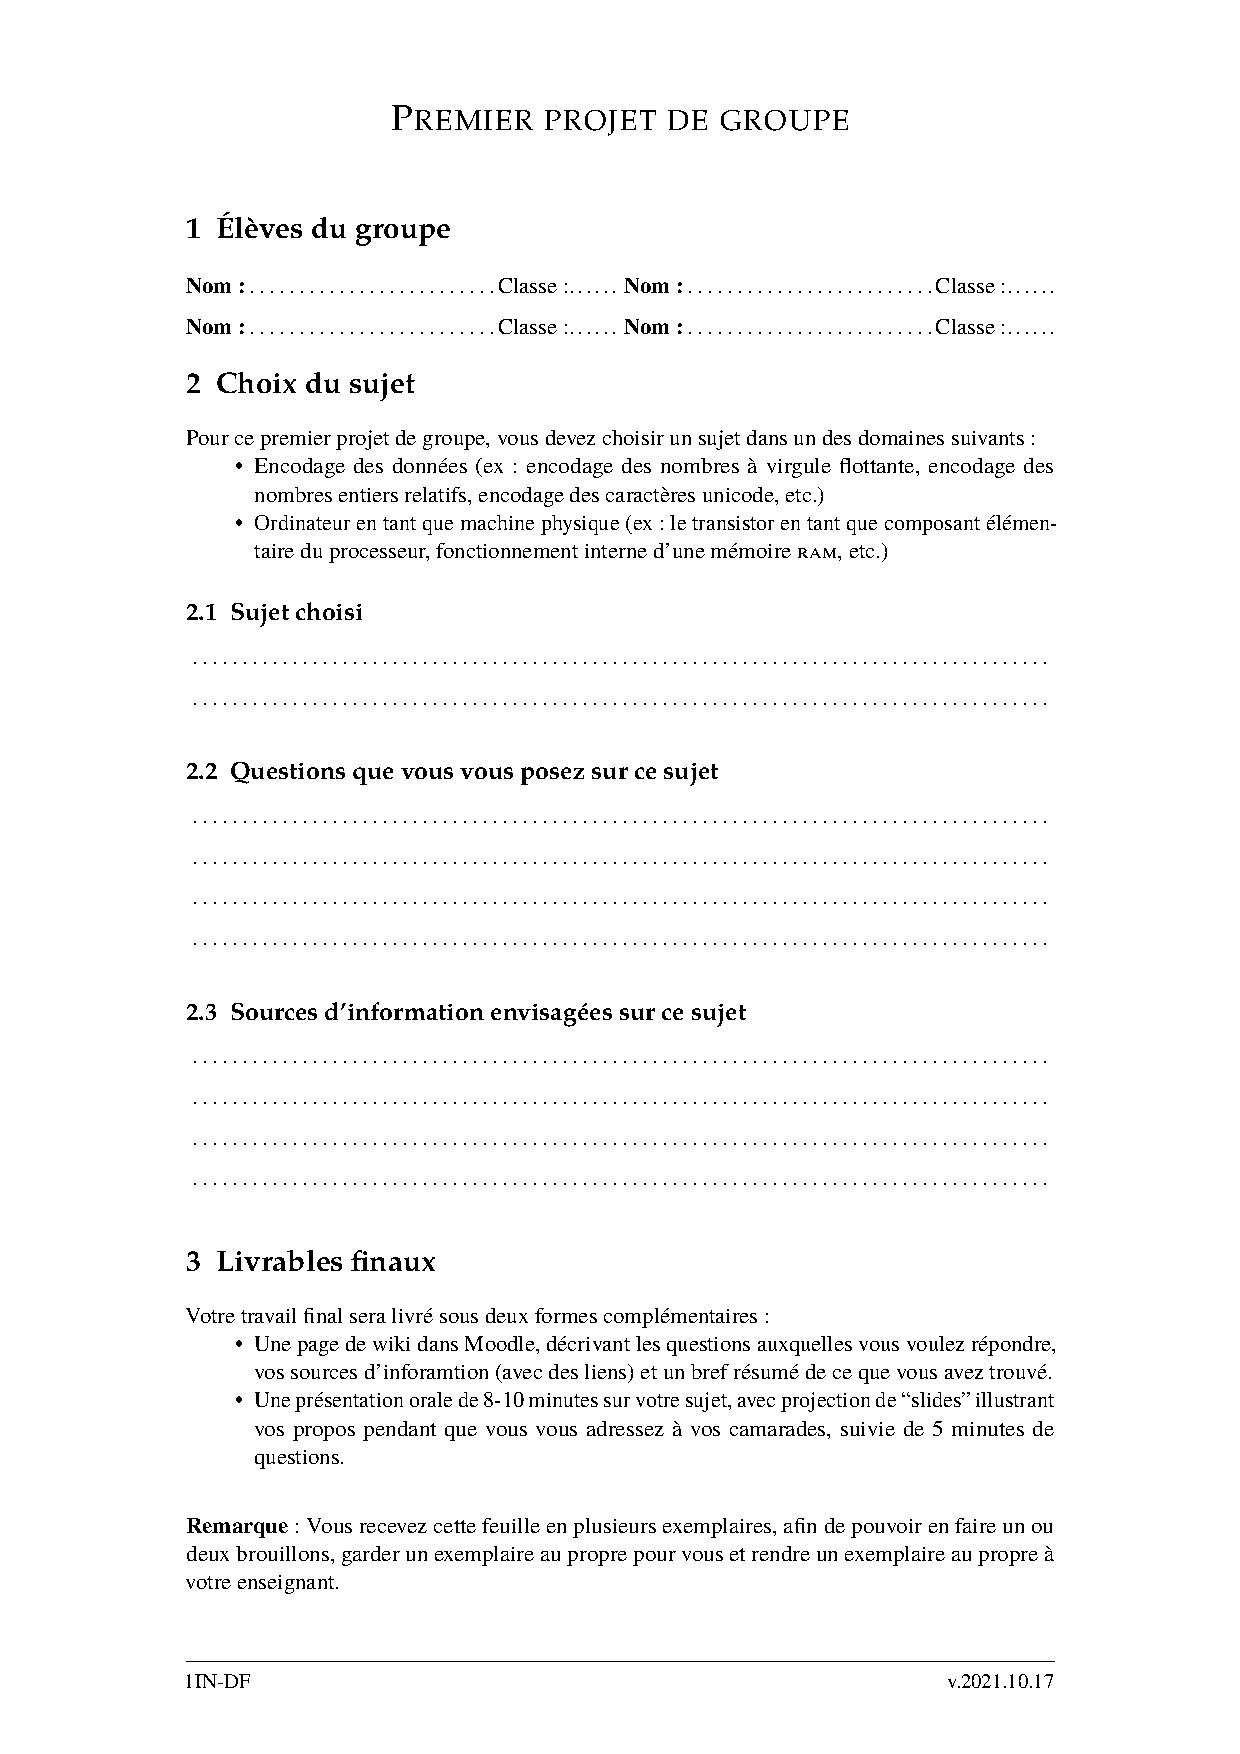
\includegraphics[width=.95\textwidth]{annexes/projet1.pdf}

\annexe{\rajout{Exemple de calendrier}}
\label{annexe:calendrier}
\begin{center}
  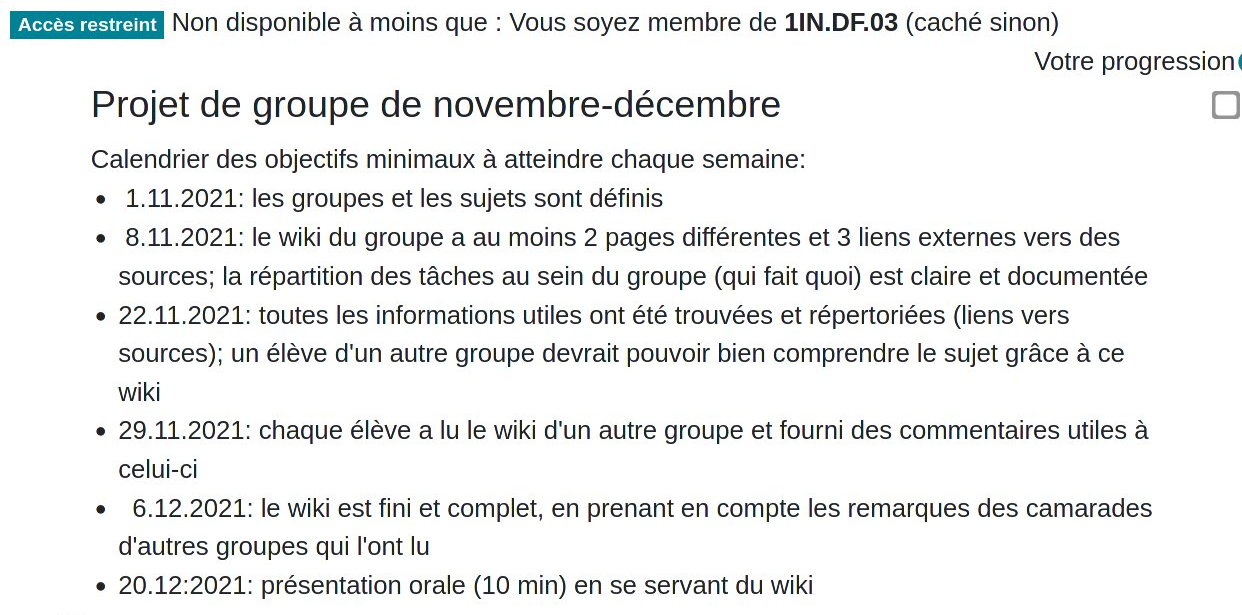
\includegraphics[width=.9\textwidth]{annexes/calendrier.png}
\end{center}

\annexe{Évaluation par les pairs} % pas numéroté, pas au toc
\label{annexe:pairs}
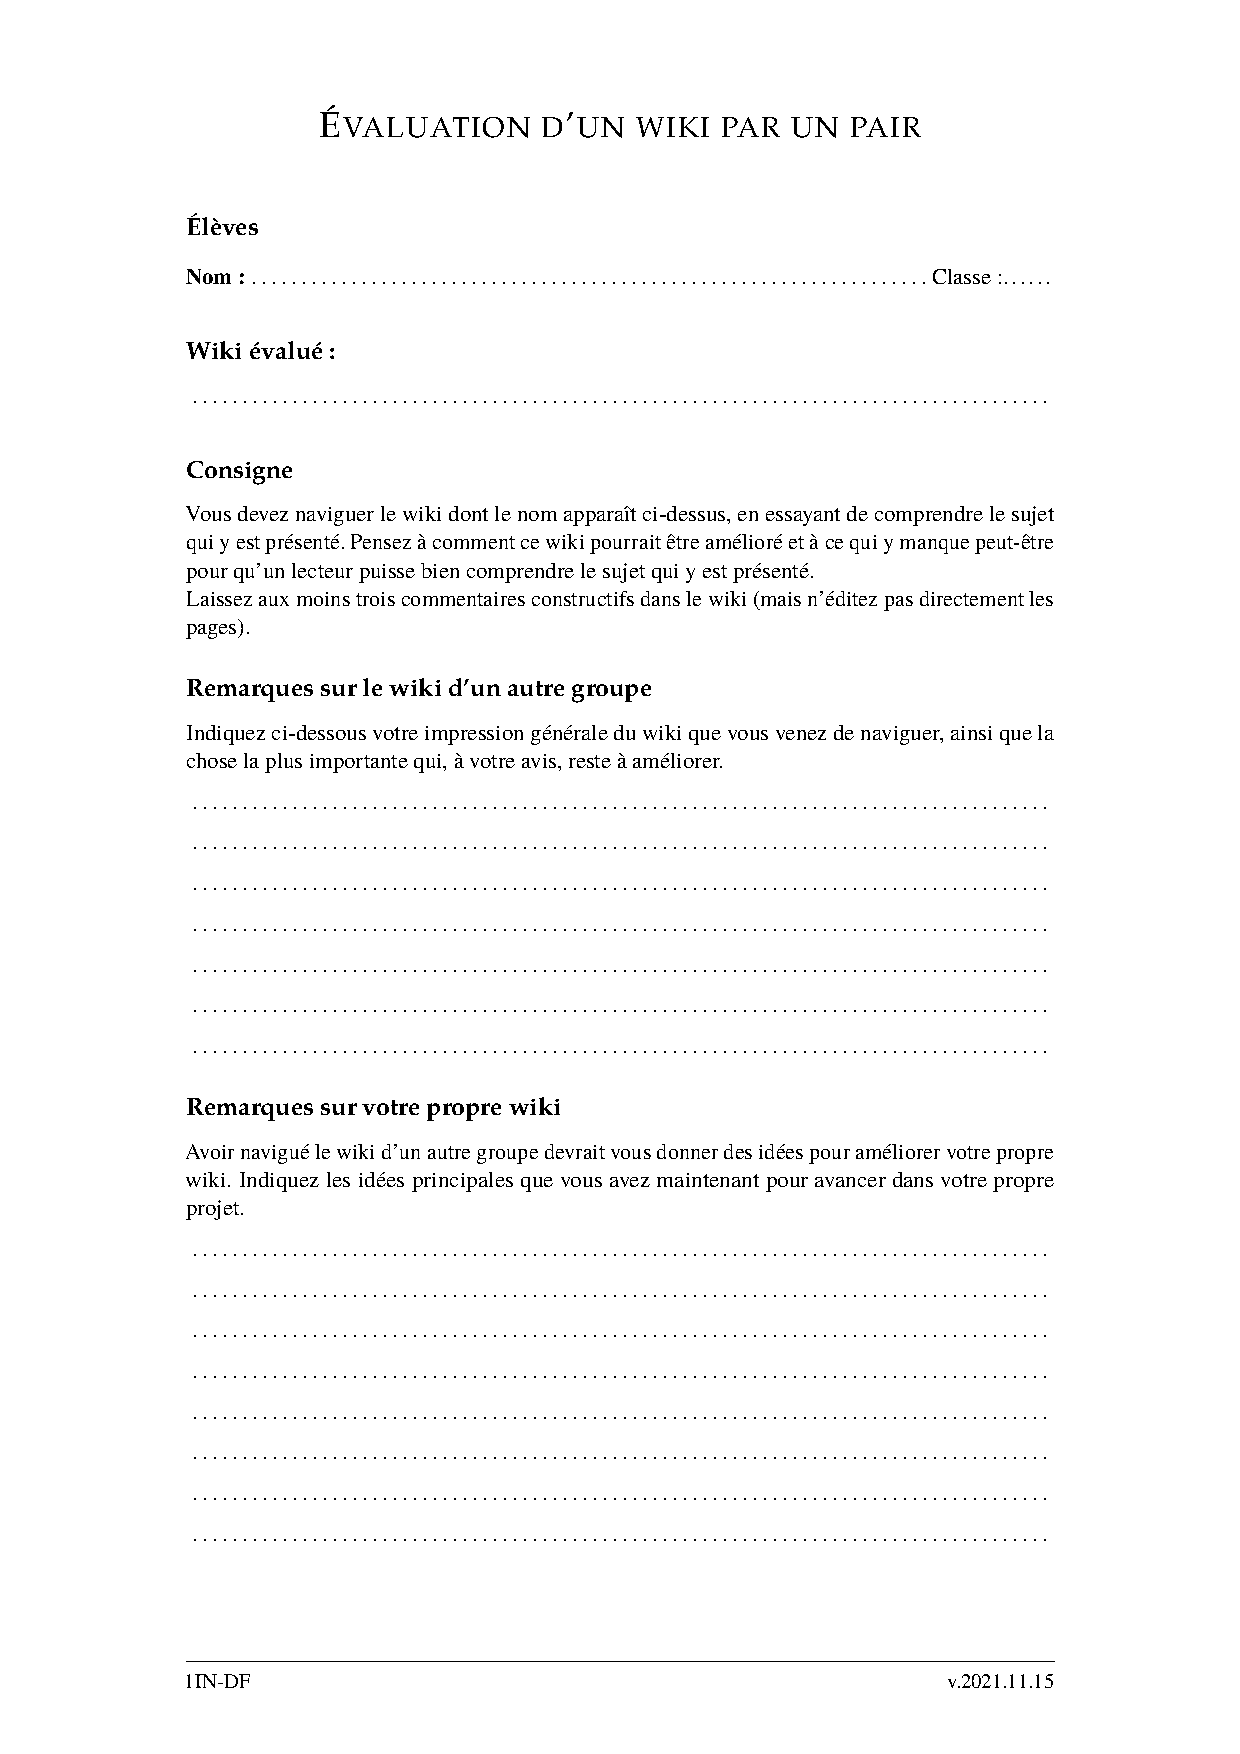
\includegraphics[width=.95\textwidth]{annexes/pairs.pdf}

\annexe{Grille d'évaluation du projet} % pas numéroté, pas au toc
\label{annexe:grille}
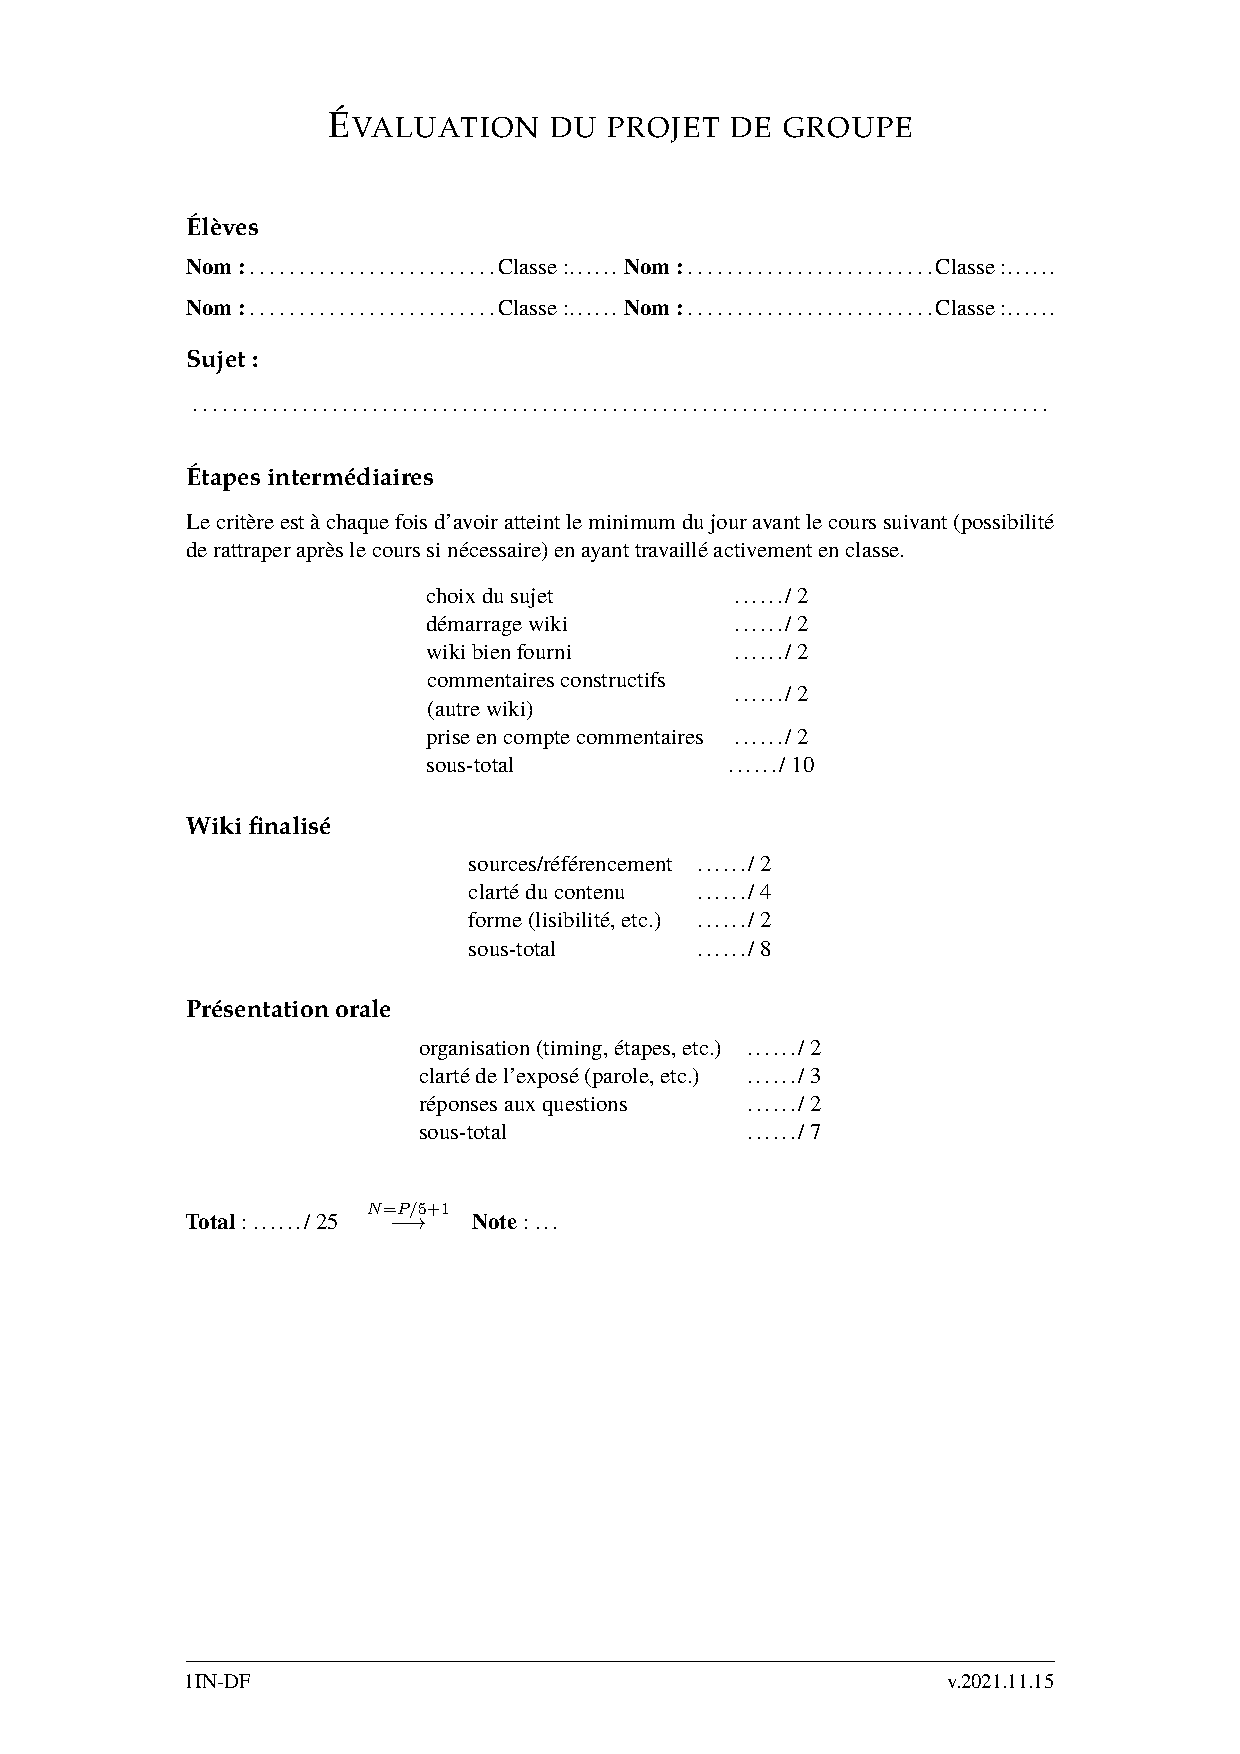
\includegraphics[width=.95\textwidth]{annexes/evaluation.pdf}

\end{document}